\subsection{Optimization of the QUBO formulation using classical heuristics}

In this Section we present the result for the optimization of the QUBO
formulation of the ATM problem using the Isoenergetic Cluster Method (a
rejectionfree cluster algorithm for spin glasses that greatly improves
thermalization) \cite{zhu2015}, which has been shown to be one of the fastest
classical heuristic to optimize QUBO problems \cite{mandra2016}.\\

Figure~(\ref{fig:icm1}) shows the total delay time optimized by ICM either by 
varying the partition at fixed the delay step $\Delta t$ (left panel) or by
varying the delay step $\Delta t$ at fixed partition (right panel). As one can
see, the total delay decreases by decreasing $\Delta t$ and it eventually
reaches an optimal plateau. Results are for maximum delay of 60 minutes. This is
consistent with the idea that smaller $\Delta t$ allows a finer optimization of
the delays of the flights.\\

\begin{figure*}
  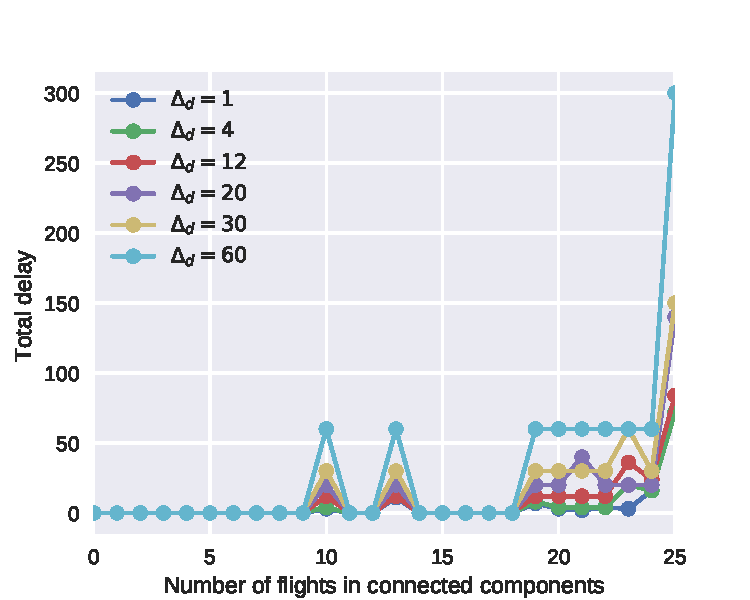
\includegraphics[width=\columnwidth]{pics/qubo_icm/qubo_icm_3.pdf}
  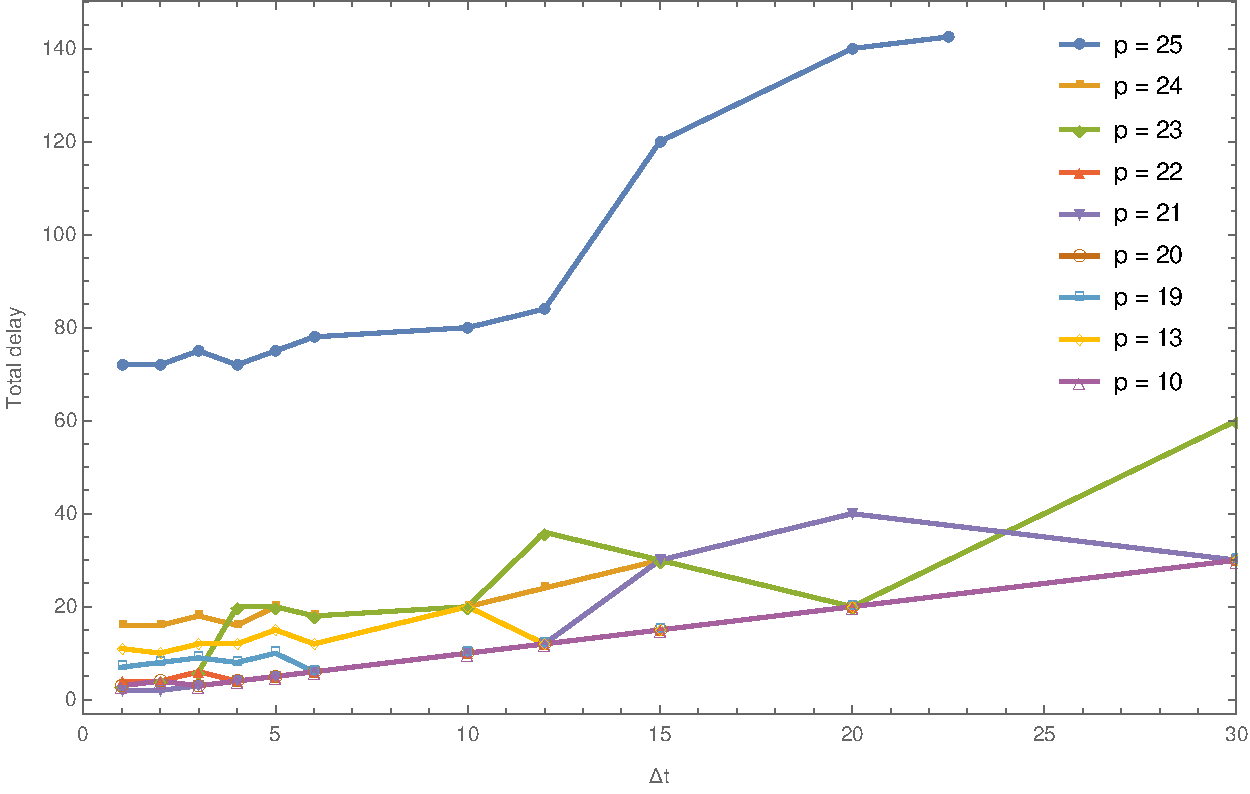
\includegraphics[width=\columnwidth]{pics/qubo_icm/qubo_icm_4.pdf}
  \caption{\label{fig:icm1}(Left) Optimal total delay found by using the
  Isoenergetic Cluster Method (ICM) at fixed time step $\Delta t$, by varying
  the connected component. Results are for maximum delay time of $60$ minutes. (Right)
  Optimal delay found by using ICM at fixed connected component, by varying the time step
  $\Delta t$.}
\end{figure*}

In Figure~(\ref{fig:icm2}) we show the optimal delay time found by ICM as a
function of the number of the flights in the connected components. Results are
for a maximum delay of 60 minutes. Unfortunately, ICM was unable to optimize
connected components with more than $12$ flights. This can be explained by
recalling that ICM works the best for almost-planar problem while the
its performance quickly decreases for fully-connected problems. Indeed, as shown
in Section~\ref{sec:instances}, the underlying graph of connected components
look more like a fully-connected graph rather than a tree graph by increasing
the number of flights inside the connected component.

\begin{figure}
  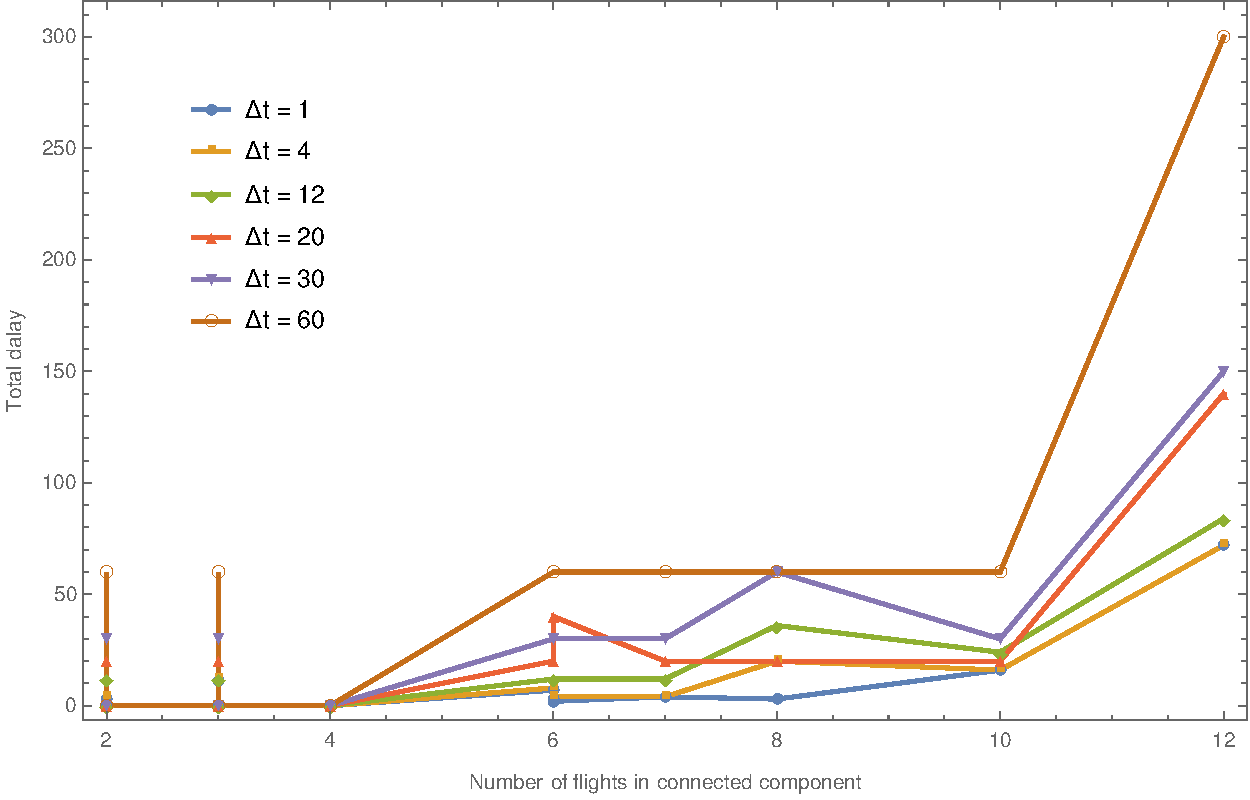
\includegraphics[width=\columnwidth]{pics/qubo_icm/qubo_icm_2.pdf}
  \caption{\label{fig:icm2}. Optimal total delay found by using the Isoenergetic
  Cluster Method (ICM) at fixed time step $\Delta t$ as a function of numbers of
  flight within each connected component. ICM was unable to find solutions for connected
  component with more than $12$ flights.}
\end{figure}
